\documentclass[10pt, a4paper]{scrartcl}

\usepackage{vorschule}
\usepackage[
	typ=ab,
	fach=Informatik,
	lerngruppe={Q1-LK} ,
	nummer=7,
	module={Symbole,Lizenzen},
	seitenzahlen=keine,
	farbig,
	lizenz=cc-by-nc-sa-4,
]{schule}

\usepackage[
	kuerzel=Ngb,
	reihe={Automaten und formale Sprachen} ,
	version={2021-03-12} ,
]{ngbschule}

\author{J. Neugebauer}
\title{Kontextfreie Sprachen}
\date{\Heute}

\setzeAufgabentemplate{ngbnormal}

\usepackage{FLaAL}
\usepackage{qrcode}

\renewcommand{\qrhinweis}[1]{%
	\begin{wrapfigure}[4]{r}{0pt}
		\qrcode[height=1cm]{#1}
	\end{wrapfigure}%
}

\begin{document}
\ReiheTitel

\begin{infobox}
\subsection*{Notation von Sprachen}
Sprachen sind Mengen von Wörtern. Um eine Sprache zu beschreiben gibt es verschiedene Notationen:
\begin{smallitemize}
	\item Umgangssprachlich: \enquote{Alle Wörter, die mit beliebig vielen \code{a} anfangen, gefolgt von genauso vielen \code{b}.}
	\item Als spezifische Menge von Wörter: $L = \{ 000, 001, 010, 011, 100, 101, 110, 111 \}$
	\item Als allgemeine Menge von Wörtern: $L = \{ w | \text{w ist ein Palindrom} \}$
	\item Als regulärer Ausdruck: $L = a^{*}(c|b)a^{*}$
	\item Als erweiterter regulärer Ausdruck: $L = a^nb^m, \quad n,m \geq 1$
\end{smallitemize}
\end{infobox}

Eine Sprache ist \emph{regulär}, wenn sie durch einen (deterministischen) endlichen Automaten akzeptiert, bzw. durch eine (rechts)reguläre Grammatik erzeugt wird. Beispielsweise $L=a^nb^m, n,m \geq 1$:
\begin{figure}[h]
	\begin{subfigure}{.5\textwidth}
		\begin{transitiongraph}[fa]
			\state[s]{q0}{0}{0}
			\state{q1}{25}{0}
			\state[f]{q2}{50}{0}
			\transition{q0}{q1}{a}
			\transition{q1}{q1}{a}
			\transition{q1}{q2}{b}
			\transition{q2}{q2}{b}
		\end{transitiongraph}
	\end{subfigure}%
	\begin{subfigure}{.5\textwidth}
		\begin{align*}
		S &\rightarrow a A \\
		A &\rightarrow a A \,|\, b B \\
		B &\rightarrow b B \,|\, \varepsilon
		\end{align*}
	\end{subfigure}
\end{figure}

\begin{aufgabe}
\label{aufg:grammatiken-erstellen}
Erstelle Grammatiken und endliche Automaten zu folgenden Sprachen:
\begin{teilaufgaben}
	\teilaufgabe $L_1 = a^nb^m, \quad n\geq 0, m \geq 2$
	\teilaufgabe $L_2 = a^nb^n, \quad 1\leq n \leq 2$
	\teilaufgabe $L_3 = a^nb^n, \quad n \geq 1$
\end{teilaufgaben}
\end{aufgabe}

\begin{aufgabe}[symbol=\symPartner]
\label{aufg:grammatik-erweitern}
Tatsächlich gibt es keine reguläre Grammatik, die die Sprache $L_3$ aus \prettyref{aufg:grammatiken-erstellen} erzeugt.

Beschreibt möglichst präzise das Problem, warum eine reguläre Grammatik nicht ausreicht und diskutiert Lösungsansätze. Wie könnte eine Grammatik zu $L_3$ aussehen, wenn die Produktionen keinen Einschränkungen unterliegen?
\end{aufgabe}

\hrulefill

\begin{wrapfig}
\begin{wrapfigure}[12]{r}{0pt}
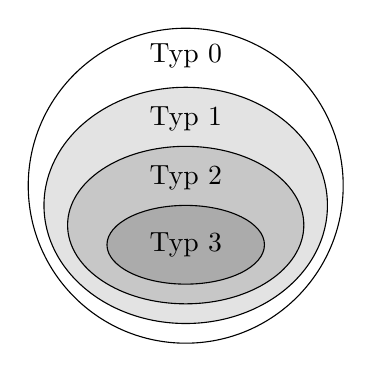
\begin{tikzpicture}
	\draw[fill=white] (0,.75) ellipse (2cm and 2cm);
	\draw[fill=black!11] (0,.5) ellipse (1.8cm and 1.5cm);
	\draw[fill=black!22] (0,.25) ellipse (1.5cm and 1cm);
	\draw[fill=black!33] (0,0) ellipse (1cm and .5cm);
	
	\node at (0,0) {Typ 3};
	\node at (0,.85) {Typ 2};
	\node at (0,1.6) {Typ 1};
	\node at (0,2.4) {Typ 0};
\end{tikzpicture}
\caption*{Darstellung der Chomsky-Hierarchie}
\label{abb:chomsky}
\end{wrapfigure}
Die Sprache $L_3$ ist ein Beispiel für eine nicht-reguläre Sprache. Formale Sprachen lassen sich in eine Hierarchie mit vier Ebenen einsortieren. Jede Ebene ist Teil der darüber liegenden (eine Typ 2 Sprache ist auch eine Typ 3 Sprache).

\begin{smallitemize}
	\item[Typ 0] \emph{Rekursiv aufzählbare Sprachen}: Sprachen ohne Einschränkungen. Sie sind äquivalent zu \emph{Turingmaschinen}.
	\item[Typ 1] \emph{Kontextsensitive Sprachen}: Sprachen, deren Produktionen vom \enquote{Kontext} abhängen können, in dem sich ein Nichtterminal befindet.
	\item[Typ 2] \emph{Kontextfreie Sprachen}: Sprachen, deren Produktionen keine Einschränkungen haben, aber vom \enquote{Kontext} unabhängig sind.
	\item[Typ 3] \emph{Reguläre Sprachen}: Sprachen, die zusätzlichen Einschränkungen unterliegen.
\end{smallitemize}
\end{wrapfig}

\end{document}